\chapter{Related work}

\section{Introduction}

In this chapter, we introduce a few related works and papers that align with concepts described in this dissertation. The language Elm for example describes in detail the challenges of functional reactive programming, tackling many of the same problems and describing similar solutions as encountered in FrDataFlow. Despite the similarities, the difference in platforms (Elm has to adhere to the limitations of the JavaScript execution engine in browsers, while FrDataFlow is constrained to the limits of the Racket runtime) has a significant impact on the potential to parallelization. 

\section{Reactive programming}

\subsection{Elm}

In 2012, Evan Czaplicki wrote his dissertation on Elm \citep{czaplicki_elm:_2012}, a functional reactive programming language for the web. In this paper, he presents a new language \textit{Elm} that supports concurrent functional programming for the web. Elm is compiled down to JavaScript using a compiler written in Haskell and promises to produce no runtime errors when everything compiles. 
Most of the reactive programming concepts in FrDataFlow were actually heavily inspired by Elm, such as \textit{signals} and the \textit{lift} function. 
Another concept inspired by Elm is signal graphs: reactive primitives as nodes and value flows as edges. Of course, source signals are a bit different in the web. For example, Elm provides source signals that represent mouse clicks, mouse positions or generally any kind of DOM event which is captured by the standard library. In the isolated, experimental little world of FrDataFlow, primitive source signals other than the current time were hard to come by. 

\subsubsection{Order of events}

Looking at a signal graph, it is easy to imagine the parallel execution of the nodes. However, the order of events is very important. 
Take for example the signal graph shown in figure \ref{fig:relatedwork-elm-eventsorder}.

\begin{figure}[h!]
	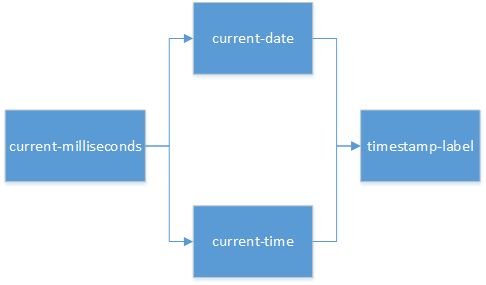
\includegraphics[width=\textwidth]{images/RelatedWork-Elm-EventsOrder.png}
	\caption{The current timestamp is based on two different computations of \textit{current-milliseconds}}
	\label{fig:relatedwork-elm-eventsorder}
\end{figure}

If a new value appears for current-milliseconds (the number of milliseconds since 1 Jan 1970), we compute the current date and current time separately, to combine these two data points into a single label called \textit{timestamp-label}. Imagine now that the computation of the current time takes significantly longer than the computation of the current date. In fact, we can contemplate that the derivation of the time would actually need to derive the date first, and then use the remaining milliseconds from midnight to determine the time. Of course, depending on the date and the timezone, this could result in different clock times.
This leads us to conclude that the calculation of \textit{current-time} is slower than \textit{current-date}. 

Now imagine that these computations are run in parallel and that their outputs are piped to the timestamp label as fast as the hardware allows it. If the date is so much faster to process, it becomes possible that the timestamp label starts receiving more than one \textit{current-date} for every \textit{current-time}, leading to situations where the date and time that shown do not both trace back to the same value of \textit{current-milliseconds} they were derived from. 

In Elm, this problem was fixed by the introduction of a global event dispatcher, which imposes a few constraints on the signal graph update loop:

\begin{itemize}
	\item Signals with more than one parent must wait for all parents to produce a value before recomputation happens. This is the same approach taken in FrDataFlow. 
	\item When source signals emit a new value, all nodes receive that event and pass forward a "nothing changed" notification. In FrDataFlow, the approach is to simply push the current value. 
\end{itemize}


\subsubsection{Parallelization}

In Elm, the constraints of the platform are slightly different. The JavaScript does not really provide native parallelization\footnote{Web workers exist, which were designed to be run in parallel. However, they come with two rather expensive limitations, the first being that messages between workers must be primitive data types, so there is no support for passing along functions with closures, only simple messages such as strings or numbers. Secondly, these web workers directly map to operating system threads, making them quite expensive to set up and tear down. The end result is that these workers are not a good fit for the small, atomic computations we are dealing with in reactive nodes.}.

Elm does provide some workarounds for 


\section{Dataflow Model}



